\section{Results}

{{For a watertight shell model,}} both its inner and outer boundary need to be supported by a huge amount of materials in order to guarantee a fine surface quality. See Figure \ref{fig:dear-simulation} (a-b) for an illustration of the Sculpture model, both its inner and outer surface require a significant amount of support in order not to be deformed during the printing process; while our approach only keeps all cylindrical shells that are free of support (Figure \ref{fig:dear-simulation} (c-d)).

\begin{figure}[t]
  \centering
  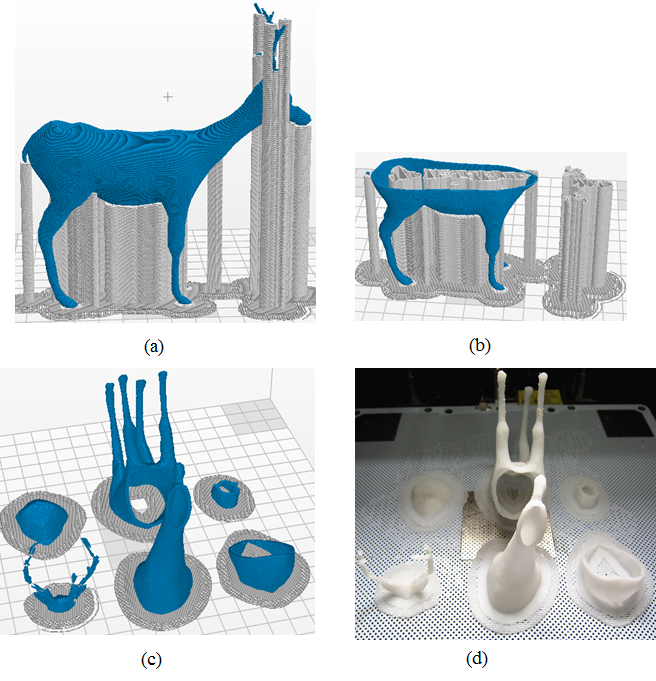
\includegraphics[width=\linewidth]{figs/dear-simulation.png}
  \caption{\label{fig:dear-simulation}%
           An illustration of the Sculpture model under the 3D printing software Z-suite as $\theta = 20^{\circ}$: (a) the full model; (b) an intermediate step of the simulation; (c) the simulation result of our partition for the Sculpture model; (d) the 3D printed result of our partition for the Sculpture model, no support is required except for the bed (limited by FDM technique).}
\end{figure}


\begin{figure}[t]
  \centering
  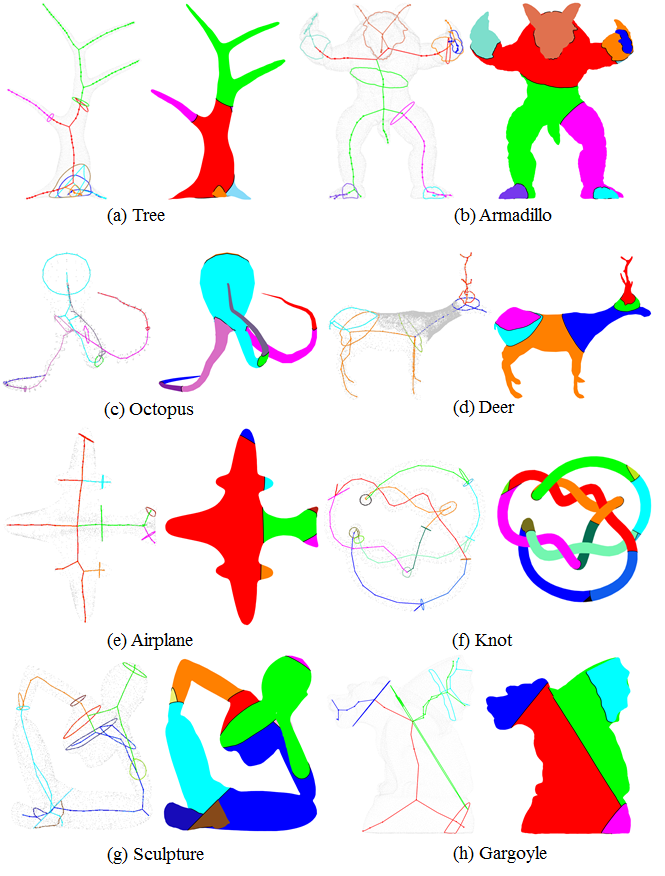
\includegraphics[width=0.45\textwidth]{figs/programming.png}
  \caption{\label{fig:programming}%
           Partition examples as $\theta = 70^{\circ}$. The printing direction of each part is orthogonal to its base (shown in the same color as the part)}
\end{figure}
We have run our algorithm on various natural or man-made models, and some of the results are presented in Figure \ref{fig:experiment}. We validated our approach by a set of printing experiments on Zortrax desktop printer, a kind of FDM machine that allows a printing layer thickness of 0.09mm , this is also the layer thickness we used in the printing experiments. The experiments are based on the choice of $\theta = 70^{\circ}$, i.e., all overhangs with an angle of no larger than $20^{\circ}$ with respect to the build platform are given support structures. Zortrax provides a built-in 3D printing software called \emph{Z-suite} that can automatically counts the filament of the print material (in meters) and an estimate of the weight of the print material. For comparison purpose, we use Meshmixer software provided by Autodesk to determine the optimal printing direction that yields the minimum amount of support materials. Table \ref{tab:ertms:summary} summarizes the printing material and time that are consumed by the original models and our partitioned models. Our approach significantly reduces both the printing material and time as the skeleton-based partition reduces both the supported materials inside and outside the models.


\begin{table*}[htb]

\begin{footnotesize}

\begin{center}

    \begin{tabular}{p{1cm} p{2cm} p{2cm} p{1.6cm} p{1.6cm} p{1.5cm} p{1.5cm} p{1.5cm} p{1.5cm}}

    \hline

     Models& Print material (original)& Print time (original)& Number of parts (skeleton partition)& Number of parts (mesh partition)& Print material (partition)& Print time (partition)& Material save (\%) &Time save(\%)\\ \hline
     Tree& 8.78m (21g)& 4h 59min &6 & 8 &5.19(12g) & 4h 2min & 35.6877 &34.4173\\ \hline
     Armadillo& 6.77m (16g)& 3h 54min &9 & 10  &4.65(11g) & 3h 30min & 39.6104 &33.3333\\ \hline
     Octopus& 13.93m (33g)& 7h 40min &5 & 9  &8.75(21g) &6h 51min & 38.8539 &37.3476\\ \hline
     Deer& 11.39m (27g)& 6h 25min &4 & 6  &8.89(21g) &5h 25min & 15.4943 &39.1386\\ \hline
     Airplane& 7.27m (17g)& 3h 56min &5 & 7 &5.24(12g) &3h 10min & 20.3647 &44.4444\\ \hline
     Knots& 21.89m (52g)& 13h 35min &10 & 15 &12.38(29g) &11h 20min & 42.2844 &32.0679\\ \hline
     Sculpture& 25.92m (62g)& 13h 44min &4 & 10 &16.35(39g) &11h 23min & 25.1716 &39.0723\\ \hline
     Gargoyle& 6.2m (15g)& 3h 21min &4 & 5 &5.16(12g) &3h 48min & 23.5556 &28.3019\\ \hline

  \hline

    \end{tabular}

\end{center}

\end{footnotesize}

\caption{Statistics showing the print material, print time and partition number of the printed models.}\label{tab:ertms:summary}

\end{table*}


\begin{table*}[htb]

\begin{footnotesize}

\begin{center}

    \begin{tabular}{p{2.3cm} p{1.45cm} p{1.45cm} p{1.5cm} p{1.5cm} p{1.5cm} p{1.5cm} p{1.5cm}p{1.5cm}}

    \hline

     Models& Tree& Armadillo& Octopus& Deer& Airplane& Knots &Sculpture & Gargoyle\\ \hline
     number of vertices & 11443   & 34594   & 1343    & 8917  & 15485 & 2904    & 5979    &25002 \\ \hline
     running time(s)    &197.1732 & 311.559 & 97.1395 &90.618 &88.744 & 92.4798 &74.2186  &199.893 \\ \hline

  \hline

    \end{tabular}

\end{center}

\end{footnotesize}

\caption{The running time of processing the models.}\label{tab:ertms:time}

\end{table*}




\begin{figure}[tbp]
  \centering
  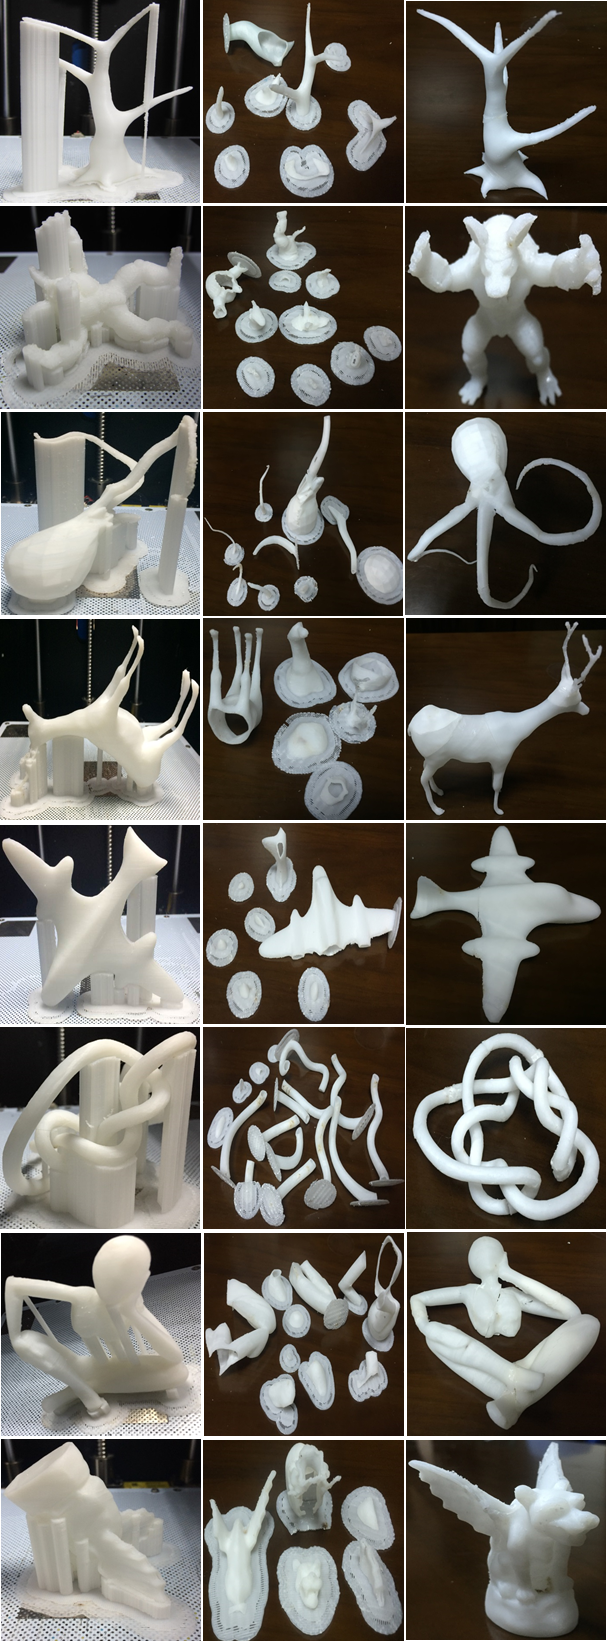
\includegraphics[width=0.48\textwidth]{figs/experiment.png}
  \caption{\label{fig:experiment}%
           A comparison between printing of original shell models and our partitioned models.}
\end{figure}

The algorithm was implemented with C++ on a PC with Intel i7-4790 and 8 GB RAM. The algorithm is run on each model for 8000 runs with the first 1000 runs taken as a training-and-learning process, the running time and the number of vertices of the models are summarized in Table \ref{tab:ertms:time}. Figure \ref{fig:experiment} shows the comparison of the printing effects of the original models and our partitioned models. Due to the limit of the current technology, any FDM printer requires a small amount of supporting bed for holding the printed model on the printing platform, other printing techniques such as SLA, SLM and SLS may avoid the use of these supporting beds. Therefore, our approach guarantees support-free to the most extent for all existing printing techniques.

Since the partition of $S$ may have exponential amount of choices, it is impossible to obtain an optimal mesh partition in polynomial time. Particularly, which arcs to be taken into a subgraph and the taking sequence significantly affect the partition result. Thus, it is hard even for our humans to determine the optimum solution. However, from Table \ref{tab:ertms:summary}, we can conclude that the partition numbers for the skeletons and mesh models are sufficiently small. Further, we can evaluate our partition result by examining some simple examples as shown in Figure \ref{fig:simpletree}.

In practice, most natural mesh models (shells) are round in the sense that there is no flat platform for supporting it on the ground, and therefore at least one cut is required. Refer to the 8-shaped model and the tree-liked model in Figure \ref{fig:simpletree}, our algorithm partitions each model into two parts (shown in red and blue respectively) with one cut, and is therefore optimal.

\begin{figure}[tbp]
  \centering
  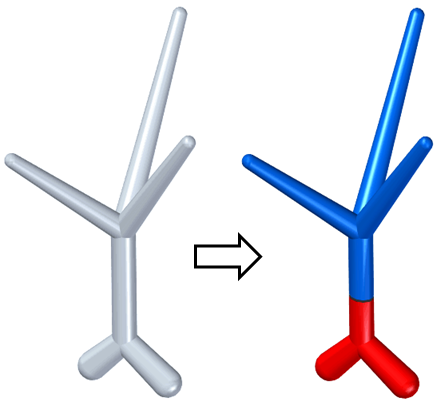
\includegraphics[width=0.5\textwidth]{figs/simpletree.png}
  \caption{\label{fig:simpletree}%
           An 8-shaped model (a) and a simplified tree model (b) that are partitioned into the least pieces by our algorithm. The printing directions are indicated by arrows.}
\end{figure}


%Further, our current approach of partitioning tries to find a node as a root of a subgraph, while in general it is possible that the subgraph is unrooted. For example, in Figure \ref{fig:unrooted}, under the angle constraint of $\theta = 70{\circ}$, the tree skeleton can be taken as a whole printable graph while our algorithm would take node $v$ as a root for the upper and lower parts of the tree respectively. Future research can be elaborated along this line. But how the general unrooted subgraphs are taken efficiently other than  searching in an exhaustive combinatorial manner to form a minimum set of subgraphs is unknown.

%\begin{figure}[tbp]
%  \centering
%  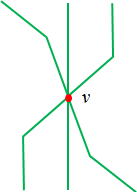
\includegraphics[width=0.2\textwidth]{figs/unrooted.png}
%  \caption{\label{fig:unrooted}%
%           An illustration of a tree skeleton that satisfies the angle constraint but is taken as two subgraphs by our algorithm.}
%\end{figure}

%However, we can evaluate the effectiveness of our approach by judging the topology of some simple models and evaluate how close our partition is from a potential optimal result. For example, from Figure \ref{fig:ex1}, under the requirement of $\theta = 70^{\circ}$, ignoring the tinny detailed geometric features we can observe that an optimal partition of the deer model requires at least $4$ cuts: the tail, the chunk including the legs, the neck, and the head and the horn. Our approach provides a partition of 4 cuts, which is almost near the optimal. Further, from the appearance of the gargoyle model (the last row of Figure \ref{fig:experiment}), we can see that an optimal cutting should have the following 4 parts: the head, two wings, and the remaining parts. Our partition results in 5 parts, which is very close to the potential optimal partition.

%Our approach is devoted to shell models, it can also be applied to cutting solid models without any problem. However, our approach suffers from a few limitations: for shell models, the thickness of the shells need to be large enough such that no serious deformation is caused during the assembling process. However, the problem of setting the minimum thickness of the model for various parts of the model is non-trivial, and our current work is restricted to a uniform setting of the shell thickness whose value is determined by an error-and-trial process. Further, the strength guarantee is not elaborated in this work, a possible solution is to use the algorithm in \cite{WangWYLTTDCL13} that distributes the least amount of materials for constructing a truss frame beneath the skin. Finally, our approach may allow a cut that passes through a salience region, which may hurt the appearance of the model. We found that it is difficult to make a balance between the saliency and the minimal cutting length as well as the minimal cutting numbers. A potential future research is to take care of salience region during graph partition. Finally, as a trade-off, a spatially curved cut might be a consideration to alleviate the salience problem.
